\chapter{Problems\ldots and solutions!}
%--------------------------------------

This chapter contains a list of Frequently Asked Questions concerning many aspects of \diva as well as a list of solved issues or bugs.

\minitoc


\section{FAQ}

\subsection{Where can I find the latest version?}
%--------------------------------------------------

\index{Download}
The latest stable version if available at \url{http://modb.oce.ulg.ac.be/mediawiki/index.php/DIVA#How_to_get_the_code.3F}. 

%Another possibility is to check the page \url{http://modb.oce.ulg.ac.be/viewsvn/}, which contains the svn repository.

\subsection{What do I need to install DIVA?}
%--------------------------------------------

Check Chapter~\ref{chap:installation} where the requirements and the procedure are described.


\subsection{Is there a graphical user interface?}
%--------------------------------------------------

Previously, an interface for the 2-D version was available, but is was not up-to-date with respect to the developments of the code.

Usually, one wants to perform a large number (more than 100) analysis in order to produce a complete climatology. To this end, it is easier to use command line than to click and wait 100 times.

For the users not familiar with shells and scripts, the web interface \citep{BARTH10} can be tried at \url{http://gher-diva.phys.ulg.ac.be/web-vis/diva.html}

\subsection{Can I use \diva to interpolate measurements from satellite?}
%------------------------------------------------- 

Yes, it is always possible to perform an interpolation with \diva on this kind of data. However, a better solution is to take into account not only a single satellite images, but also the information contained in the images of the previous days. This is done with the software DINEOF \citep[e.g.,][or \url{http://modb.oce.ulg.ac.be/mediawiki/index.php/DINEOF}] {ALVERA05,BECKERS06}. 



\subsection{How to report a bug or a problem?}
%----------------------------------------------

The preferred option is to send a message to the \diva user group on google:\\
 \url{http://groups.google.com/group/diva_users}. 
 
This has two advantages over emails:
\begin{enumerate}
\item The questions is directly sent to all the \diva developers.
\item The issues previously solved are archived and available for other users.
\end{enumerate}

Along with a small description of the problem, add relevant informations that would help us solving your issue:
\begin{itemize}
\item the version of \diva you are using,
\item your operating system (O. S.),
\item your options for compiling the code\\
 (check file \file{compilation.log} in directory \directory{DIVA3D/src/Fortran/}.
\end{itemize}
If the problem can be reproduced at the 2-D level (i.e., working in the directory \directory{divastripped}), add the input files that generated the problem as well, so that we can check if the issue is machine-dependent. 

To know your O. S. you can type in the shell:

\begin{lstlisting}[style=Bash]
gherulg$ uname -voi
28-Ubuntu SMP Tue Oct 9 19:31:23 UTC 2012 x86_64 GNU/Linux
\end{lstlisting}

If you received advice which helped you to solve the problem, please post a comment so that others know the solution worked. 
%%


\subsection{How to register to the user group?}
%------------------------------------------------
\begin{itemize}
\item Go to \url{http://groups.google.com/group/diva_users} and login with a google account (not necessarily a gmail address). 
\item Follow the "\textit{Apply for membership}" link. You will be asked to explain why you want to use \diva.
\item Finally click on the "\textit{Apply to join this group}" button. \\
You will get an email confirmation once the the application has been reviewed and accepted.
\end{itemize}
 


\subsection{How can I use \diva in R, Matlab, IDL, Ferret or any other software}
%------------------------------------------------
There are basically two ways:

\subsubsection{a) Using special binaries and preparing {\tt fort.*} files for \diva}

This approach has been taken in the incorporation of \diva into ODV\index{Ocean Data View} and in the \matlab\index{Matlab} function in \url{http://modb.oce.ulg.ac.be/mediawiki/upload/divaformatlab.zip}

It requires some time (you can try to understand the matlab function to see how to prepare the files and recover the results), but has the advantage that you do not need to install \diva, compilers, NetCDF or Cygwin. It also avoids creation of large subdirectory trees for \diva. 


\subsubsection{b) Using a full \diva installation and preparation of normal \diva input files}

In this case you must have installed the \diva package and have access to either directly unix or Cygwin shells.\index{Cygwin}

You also need to prepare a shell script that we will call \command{mydivacall} in this example, and which contains the instructions to be to executed with \diva. So typically what you would type in the command-line session when trying to make the analysis.

\begin{exfile}[htpb]
\begin{footnotesize}
\begin{verbatim}
#!/bin/bash
export LC_ALL=C
PATH=$PATH:.
cd /home
pwd
echo This is a test
echo Hello Diva world
...
# Then go into the divastripped directory and run the scripts you want
\end{verbatim}
\end{footnotesize}
\caption{mydivacall\label{ex:mydivacall}}
\end{exfile}

Then your program has to prepare all input files exactly as for a normal \diva execution. Once this is done, your program needs to make a system call (look at the documentation of your program on how to do it). On a Unix machine you would then simply include a command like

\command{call system("/home/<path>/mydivacall")}

For a Cygwin system it is more complicated:

{\footnotesize
\command{call system("c:$\backslash$cygwin$\backslash$bin$\backslash$bash.exe --login -i -c c:/<path>/mydivacall")}
}
%\begin{lstlisting}[style=Bash]
%call system("c:cygwin\bin\bash.exe --login -i -c c:/<path>/mydivacall")
%\end{lstlisting}

Once the script execution is finished, you can read the diva output files with your program and continue the processing.

%\url{www.neurotap.blogspot.com.es/2010/08/how-to-call-bash-command-outside-of.html}
% add a link to the web page that explain that

\subsection{What value for parameter \texttt{ireg} should I choose for a semi-normed analysis}
%----------------------------------------------------------------------------------------------

\index{Semi-normed analysis}
The best option is to choose \texttt{ireg} = 0.

The command \command{divaseminorm} performs four operations:
\begin{enumerate}
\item \command{divarefe} = computing a reference fields with large value for $L$ (your
value multiplied by 5) and low signal-to-noise ratio (your value divided by 10)

\item \command{divaanom}: difference between your data values and the reference field at
these data points

\item \command{divacalc}: performs a \diva analysis with the parameters you put in
\file{param.par}, on the data anomaly. This is why you should choose ireg=0: you
are working with anomalies, thus no need to subtract any background field.

\item \command{divasumup}: reconstruction of the analysed field by summing the reference
and anomaly fields.

\end{enumerate}


\subsection{How can one create monthly analysis where the reference field is the annual analysis?}
%----------------------------------------------------------------------------------------------

\index{Background field}
The latest version of \command{divaanom} is able to use an existing reference field. This field should be present as a binary file in the output directory with the name \file{fieldgher.anl.ref}, and the \file{GridInfo.dat} file should be present in \directory{output/ghertonetcdf/} directory.

An execution of \command{divaanom} will provide you with \file{data.dat} which contains anomalies with respect to your reference field (annual analysis in this case). Then you can work with \file{data.dat} as usual. 

The last step is to apply \command{divasumup} to reconstruct the field by summing the anomaly analysis and the reference field.

In summary the steps to follow are:

\begin{enumerate} 
\item apply \command{divadress} to the annual data (after the optimisation of the parameters),
\item copy the output \file{fieldgher.anl} with the name \file{fieldgher.anl.ref},
\item for each month:
\begin{enumerate}
\item copy the corresponding data file into the input directory,
\item apply \command{divaanom},
\item perform an analysis on the anomalies,
\item apply \command{divasumup}.
\end{enumerate}									 
\end{enumerate}
									 
%\section{}
%
%
%longitude latitude
%coordinate system is chosen by the user, it is up to him to make the adequate projection.

\subsection{How to contribute to the development?}
%----------------------------------------------

Any suggestion concerning the development of the software is welcome. Simply send to the developers or to the google group, a description  of what improvements/tools you would like to see and we will check if this could be easily added to the general distribution.


\subsection{How can I run \diva on a multi-processor machine?}
%------------------------------------------------------------

\subsubsection{Coarse grain parallelisation}

The best option is to copy the whole directory \directory{divastripped} in the directory in which it is located, but with a different name (e.g., \directory{divastripped2}, or \directory{divastripped\_username1}). The you can run \diva analysis separately in these directories. 


\begin{figure}[htpb]
\centering
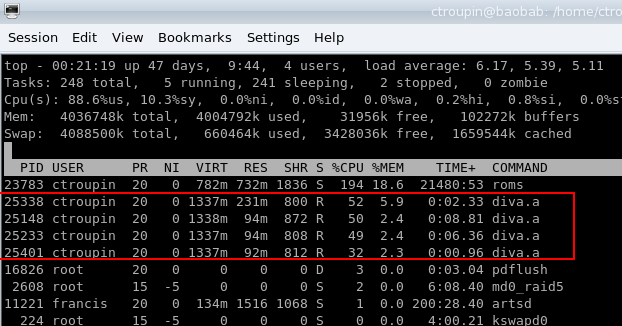
\includegraphics[width=.80\textwidth]{multiple_diva}
\caption{Simultaneous run of \diva.}
\end{figure}

\subsubsection{Fine grain parallelisation}

If you compiled \diva for parallel use, you can activate the parallel solver by editing \command{divacalc} and use \texttt{solver=1}

\subsection{What is the resolution of the output field?}
%-------------------------------------------------------

One has to distinguish between 2 \textit{resolutions}:

\begin{enumerate}
\item the resolution brought by the finite-element mesh, of which the characteristic length should be in agreement with the typical scale of the studied region (based on the data correlation in \diva);

\item the grid resolution, which can be anything (larger, smaller or similar to the mesh resolution). It means that you can always work with a finer grid, but that does not mean that the actual resolution will be improved.
\end{enumerate}

So the best resolution you can obtain is the one allowed you by the data you are working with.


\subsection{Why is there an iterative solver?}
%-------------------------------------------------------

You can activate an iterative solver by editing \command{divacalc} and use \texttt{solver=2}. This can be useful if you do not calculate error fields and do not use cross validation techniques but work with very fine grids. In this case execution time can be reduced. There are some tuning parameters which can enhance convergence but to exploit them, please contact us.


\subsection{Can \diva deal with several measurements at the same location?}
%---------------------------------------------------------------------------

Yes. In that case (for example: time series, mooring, \ldots) \diva provides an average value. 

However, when data locations are very close and values are very different and a huge signal-to-noise ratio is used, then you will see artefacts simply showing that you have created a huge gradient because you said to \diva your data are perfect and yet are very different at very close stations. Figure~\ref{fig:results_twopoints_center} provides an example of a situation with two different measurements at the same point.

\begin{figure}[H]
\centering 
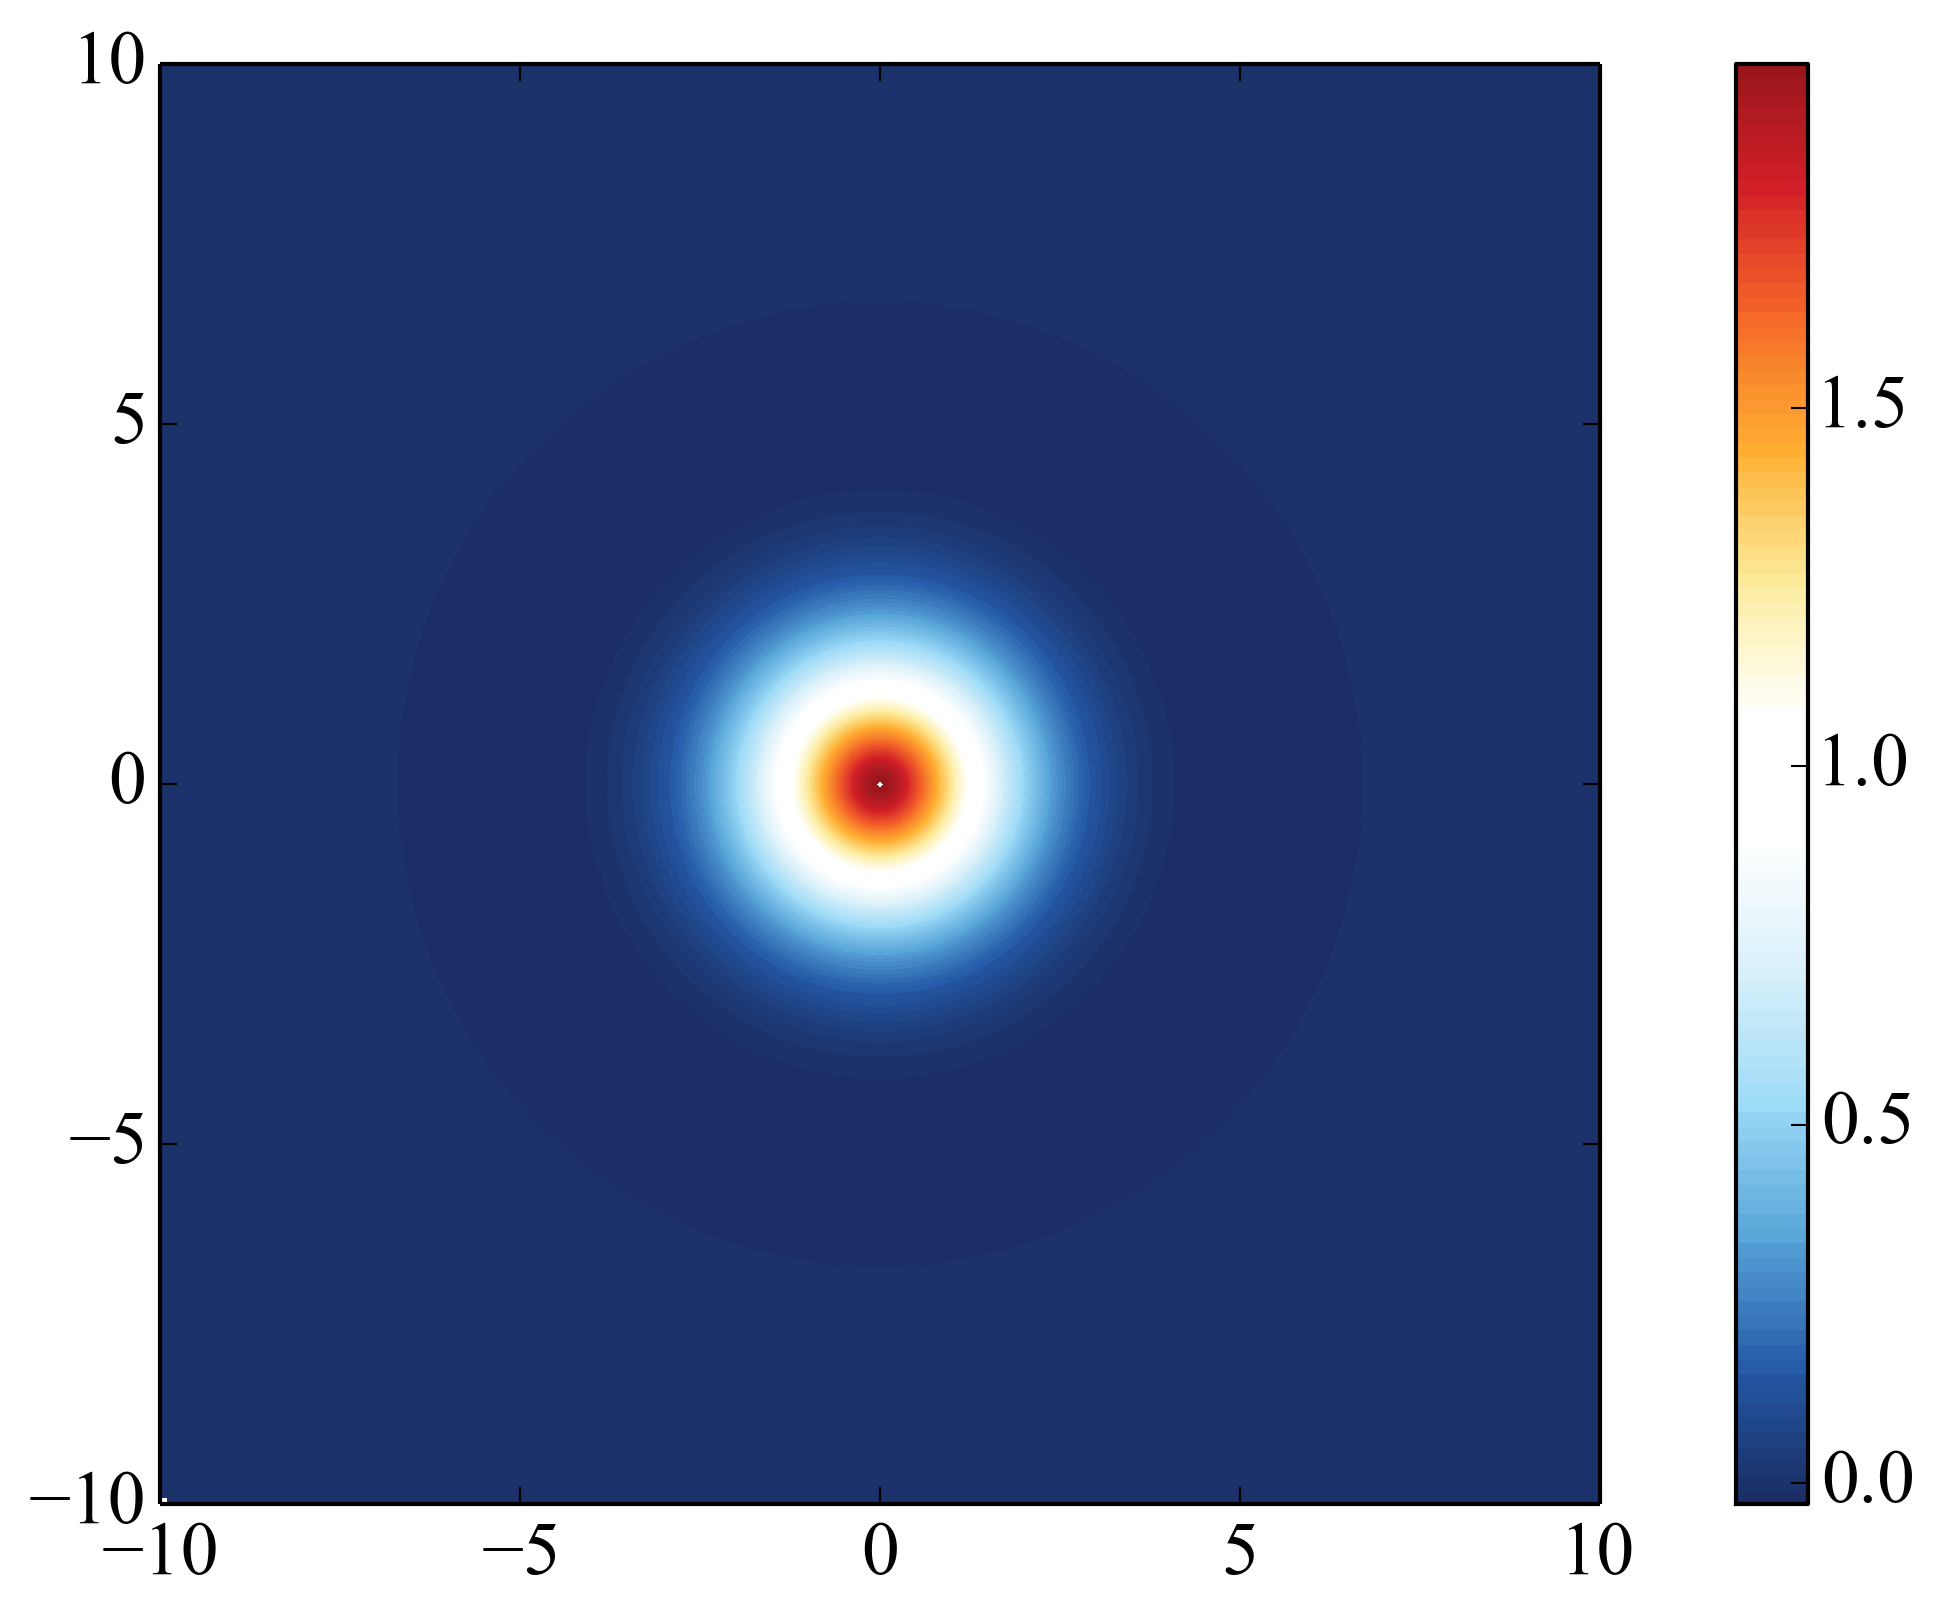
\includegraphics[width=.7\textwidth]{results_twopoints_center}
\caption[Results with two data points with values 1 and 3, located in the domain center (0,0), with a large signal-to-noise ratio.]{Results with two data points with values 1 and 3, located in the domain center (0,0), with a large signal-to-noise ratio. The analyzed field at (0,0) is $\approx 2$.\label{fig:results_twopoints_center}}
\end{figure}


\subsection{How to run \diva in operational or real-time mode?}
%---------------------------------------------------------------------------

The idea is to work on a data set that evolved regularly, let's say every day. It is assumed that the files are formatted so that they can be ingested by \diva (either ODV format for 4D runs, or simple 3-column files for 2D runs), and that a script \command{mydivarun} prepares the input files, execute \diva and copy the results into another directory.

On Unix-like computers, the software utility \command{cron} can be used to schedule a task, such as a \diva execution. Please consult the documentation relative to \command{cron} and \command{crontab}, for example: 
\url{http://ss64.com/bash/crontab.html} or \url{http://cronjob.com/}.\index{cron}

To have \command{mydivarun} executed every day at 9.15 AM, the crontab has to be edited:
\begin{lstlisting}[style=Bash]
gherulg$ crontab -e
\end{lstlisting}
and a line such as 
\begin{lstlisting}[style=Bash]
gherulg$ 9 15 * * *   path_to_scripts/mydivarun
\end{lstlisting}
is added. If everything goes well, you can skip the rest of this section.

Otherwise, if the script run properly when called directly from the shell, but not from the cronjob, it is probably due to the environment variables (PATH, LD\_LIBRARY\_PATH \ldots) passed by cron are minimal. For example your path used by cron is not the same path that you have when typing commands. To avoid this problem:
\begin{itemize}
\item Use absolute path for your commands. Note that \diva commands (\command{divacalc}, \command{divamesh}, \ldots) have to be run from the \directory{DIVA3D/divastripped/} directory. Hence in the script \command{mydivarun}, you may write something like
\begin{lstlisting}[style=Bash]
here=$pwd
divadir=path_to_divadir
cd $divadir
./divadress
cd $here
\end{lstlisting}
\item Manually add the path at the beginning of the script you want to run.
\end{itemize}

A good idea for debugging is to redirect the standard output and error in text files:
\begin{lstlisting}[style=Bash]
gherulg$ 9 15 * * *   path_to_scripts/mydivarun > path_to_directory/crontab.out 2>/home/ctroupin/DataOceano/AVISO/Operational/crontab.err
\end{lstlisting}

A list of possible reasons for cron job failure is found at\\
\url{http://askubuntu.com/questions/23009/reasons-why-crontab-does-not-work}.


%--------------------------------------------
\section{Error messages}
%--------------------------------------------



\subsection{"Command not found" message}
%------------------------------------

\begin{lstlisting}[style=Bash]
MacBook-Pro-de-GHER:divastripped gherulg$ divatest
-bash: divatest: command not found
\end{lstlisting}

%\begin{figure}[htpb]
%\centering
%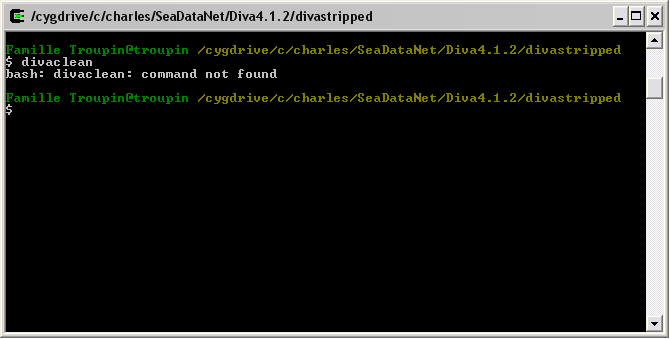
\includegraphics[width=.80\textwidth]{problempath}
%\caption{Error message when a command is not found.}
%\end{figure}

\subsubsection{\question}
%--------------------------------------

Although you are in the correct directory, the command is not found. This is because the current directory (represented by \texttt{./}) is not in the path of your system. 

\subsubsection{\answer}
%--------------------------------------

You can type \\
\command{./name\_of\_the\_command}\\
so that the system knows the command is the current directory.

A better solution is to adapt your path by typing:\\
\command{PATH=\$PATH:path\_to\_diva\_directory}, where \verb|path\_to\_diva\_directory| has to be adapted to your installation.

For example:
\begin{lstlisting}[style=Bash]
ctroupin@predator ~/Software/Diva/DIVA3D/divastripped $ pwd
/home/ctroupin/Software/Diva/DIVA3D/divastripped
ctroupin@predator ~/Software/Diva/DIVA3D/divastripped $export  PATH=$PATH:home/ctroupin/Software/Diva/DIVA3D/divastripped
ctroupin@predator ~/Software/Diva/DIVA3D/divastripped $ echo $PATH
/usr/local/sbin:/usr/local/bin:/usr/sbin:/usr/bin:/home/ctroupin/Software/Diva/DIVA3D/divastripped/
\end{lstlisting}

For example in \texttt{cygwin}:\\
\begin{itemize}
\item go in the \texttt{/ect/}
\item edit file \texttt{bash.bashrc} file
and add the following line:\\
export \texttt{PATH=\$PATH:.}
\item type \command{source bash.bashrc} in order to take into account the modification made.
\end{itemize}


%----------------------------------------------------------------------------------------------

\subsection{Analysed field with white boxes near boundaries}
%------------------------------------------

The analysed fields has points of \textit{not-a-number} ($NaN$) values.

\begin{figure}[htpb]
\centering
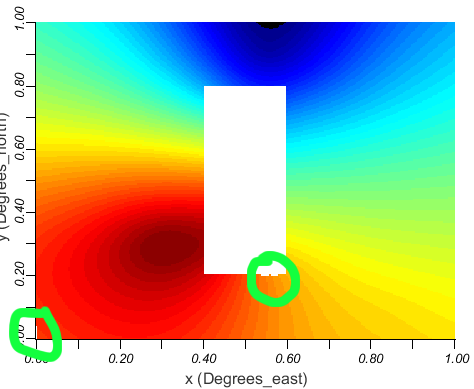
\includegraphics[width=.45\textwidth]{error_stripes_bound}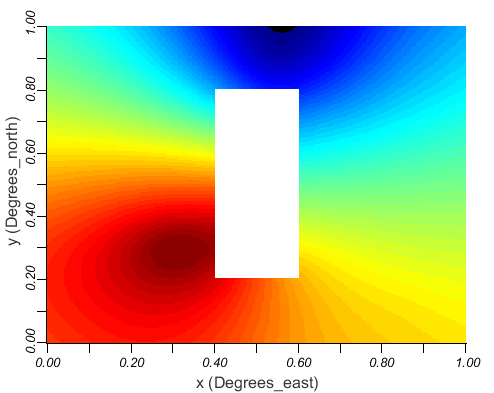
\includegraphics[width=.45\textwidth]{error_stripes_bound_corr}
\caption[Examples of \diva outputs with zones of $NaN$ at boundaries.]{Examples of \diva outputs with zones of $NaN$ at boundaries. For the right the solution to the problem was applied \label{fig:error_stripes}}
\end{figure}

\subsubsection{\question}
%--------------------------------------

This problem arises from the fact that you request the analysis almost exactly on the boundary.



\subsubsection{\answer}
%--------------------------------------

Internally \diva makes some coordinates changes and therefore roundings on boundary positions. The decision of a point falls in the domain or not can therefore be very sensitive
to rounding if you place a request for analysis "exactly" on the boundary. In real situations, this very rarely happens, but when you use synthetic test cases, use contours and analysis points which do not coincide (look at \command{divatest} how the contour is made to avoid falling on the grid points of the analysis).



\subsection{Command-line scripts not working}
%-----------------------------------------


\begin{figure}[htpb]
\centering
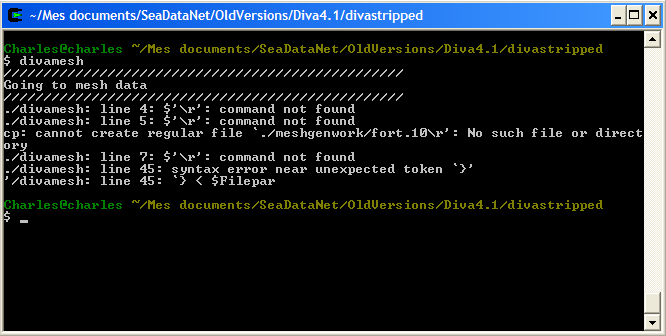
\includegraphics[width=.80\textwidth]{dos2unix2}
\caption{Error messages due to bad ends of lines. \label{fig:error_dos2unix}}
\end{figure}

\subsubsection{\question}
%--------------------------------------

End of lines in Unix,  Windows and Mac files are different, and this causes problems when switching from a system to the other. Typically if you visualize a Windows-end-of-line file under Unix, you will see ends of line with symbols such as \verb|^M| or \verb|\r|. When reading such files, scripts get in trouble because they expect to read numbers, but instead they find characters.

\textbf{Note:} strange behaviours of \diva are often related to this topic, therefore always be aware of this possible problem before undertaking more complex actions.

\begin{figure}[htpb]
\centering
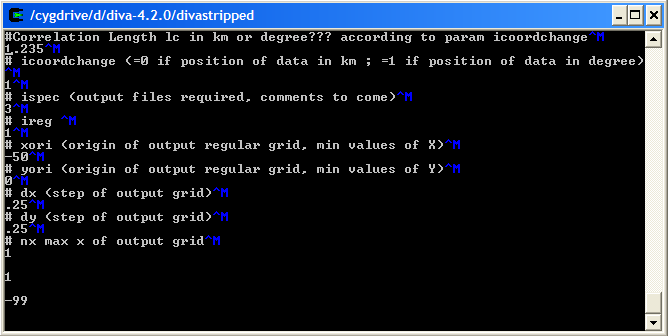
\includegraphics[width=.80\textwidth]{dos2unix}
\caption{Example of bad ends of lines.\label{fig:error_dos2unix2}}
\end{figure}


\subsubsection{\answer}
%--------------------------------------

Working on a individual file, the command\\

\begin{lstlisting}[style=Bash]
[charles@gher13 divastripped]$ dos2unix  name\_of\_the\_file
\end{lstlisting}
does the conversion between Windows and Unix end of lines. According to the Linux distribution, \command{dos2unix} may requires options to perfom the conversion. For example with Mandriva~2010, it is necessary to add the option \texttt{-U}:

\begin{lstlisting}[style=Bash]
[charles@gher13 divastripped]$ dos2unix  -U name\_of\_the\_file
\end{lstlisting}

When working with GODIVA, the transformation is automatically done on all the files. \command{dos2unix} is available using the package manager of most of Linux distributions, but sometimes with the name \texttt{fromdos}.


\subsection{Compilation problems\label{sec:error_compile}}
%------------------------------------------------------------------------------------------------

\begin{figure}[htpb]
\centering
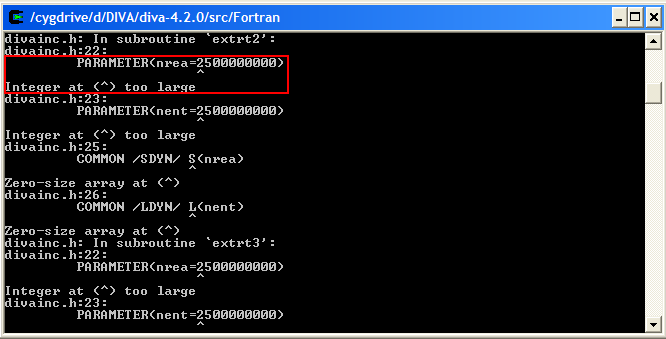
\includegraphics[width=.80\textwidth]{error_compile_g77}
\caption{Error message obtained during compilation. \label{fig:error_compile}}
\end{figure}

\subsection{\question}
%--------------------------------------

The array $S$ defined in the various programs located in \directory{./src/Fortran/Calc/} is too large to be handled by your compiler. 


\subsubsection{\answer}
%--------------------------------------

You need to recompile the sources after reducing the values of parameter \texttt{nrea} in file\\
 \file{./src/Fortran/Calc/divainc.h}:
\begin{verbatim}
      PARAMETER(nrea=150000000)
\end{verbatim}
Then use script \command{divacompile} to get the new executables (see Section~\ref{sec:compilation}). If you get the same error message, reduce again the value of \texttt{nrea}.

\begin{figure}[htpb]
\centering
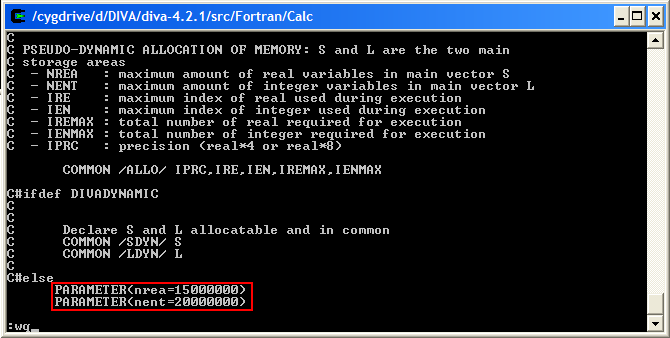
\includegraphics[width=.80\textwidth]{solution_resource}
\caption{Solution to the resource problem.}
\end{figure}


\subsection{Undefined references to NetCDF routines\label{sec:error_netcdf}}
%------------------------------------------------------------------------------------------------

\index{NetCDF}
\begin{figure}[htpb]
\centering
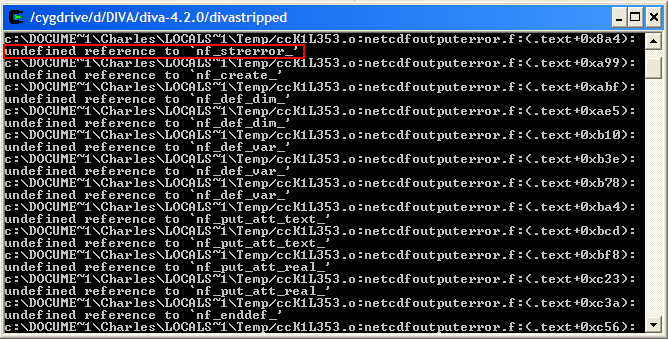
\includegraphics[width=.80\textwidth]{error_netcdf}
\caption{Error message during execution of \command{divacomp} with gfortran\label{fig:error_netcdf}.}
\end{figure}

\subsubsection{\question}
%--------------------------------------

The NetCDF library, required for compiling of \file{netcdf\-output.f}, \texttt{netcdf\-output\-field.f} and \texttt{netcdf\-output\-error.f}, is not compatible with your compiler, or not found by the linker.

\subsubsection{\answer}
%--------------------------------------

You have to make sure that \command{divacompile} includes the appropriate link path.

If this is not sufficient, you will have to rebuild the NetCDF library corresponding to your operating system. Installation and compilation procedures can be at \url{http://www.unidata.ucar.edu/software/netcdf/docs/netcdf-install/}

%----------------------------------------------------------------------------


\subsection[Resource temporarily unavailable]{Resource temporarily unavailable\label{sec:error_resource}}
%------------------------------------------------------------------------------------------------


\begin{figure}[htpb]
\centering
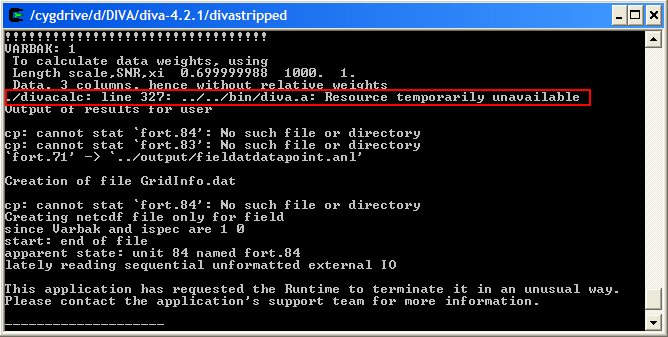
\includegraphics[width=.80\textwidth]{error_resource}
\caption{Error message during the run of \command{divacalc}\label{fig:error_resource}.}
\end{figure}

\subsubsection{\question}
%--------------------------------------

The \texttt{diva.a} executable requires to much memory to work. This error comes from the operating system limitations.

\subsubsection{\answer}
%--------------------------------------
First try to cancel all unnecessary tasks running on your machine, possibly rebooting. This will clean up the system and free up resources. If this is not sufficient, the solution is the same as case \ref{sec:error_compile}: recompile the sources after reducing the values of parameters \texttt{nrea} and \texttt{nent} in file \file{./src/Fortran/Calc/divainc.h}:
\begin{verbatim}
      PARAMETER(nrea=25000000)
      PARAMETER(nent=25000000)
\end{verbatim}
If you get the same error message, reduce again the values of \texttt{nrea} and \texttt{nent}.

Note that maximal allowable values for these parameters depends on your compiler and system, so it is not possible to assign them with universal values.

\subsection{Error of allocation \label{sec:error_allocation}}
%-------------------------------------------------------

\begin{figure}[htpb]
\centering
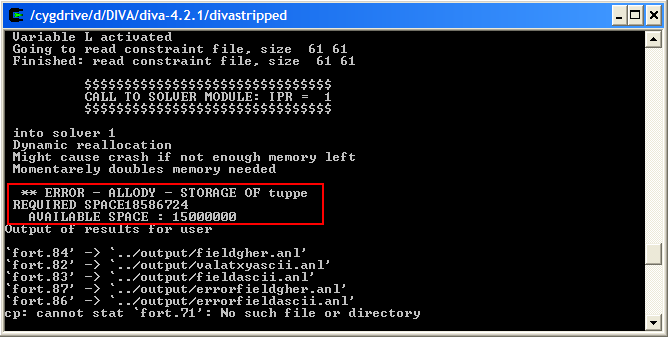
\includegraphics[width=.80\textwidth]{error_allody}
\caption{Error message due to allocation problem.\label{fig:error_allocation}}
\end{figure}

\subsubsection{\question}
%---------------------

The memory allocation is not sufficient for the \diva to be executed in the case you consider. This message may appear either during the mesh generation (the required mesh is too fine considering the size of the domain) or during the resolution itself (i.e., \command{divacalc}).

\subsubsection{\answer}
%-------------------

The solution is nearly the same as the previous case: you need to compile the source again, this time after increasing the values of \texttt{nrea} and \texttt{nent}.

\subsubsection[Additional information]{Additional information \expert}
%-------------------------------------------------------------------

In some uncommon cases, you may not be able to find values of \texttt{nrea} and \texttt{nent} that will allow you to avoid both problems \ref{sec:error_resource} and \ref{sec:error_allocation}. In these cases, the recommended solution consists of:
\begin{enumerate}
\item Find the highest values of \texttt{nrea} and \texttt{nent} that allow you not to have message error \ref{sec:error_allocation};
\item Generate a mesh with a value 3-5 times larger than the correlation length you want to use for the resolution; this can be done be simply editing file \file{./input/param.par}, changing the value of correlation length, and run \command{divamesh};
\item Once the mesh is generated, edit again \file{param.par} and assign the correct value to the correlation length, and run an analysis with \command{divacalc}.
\end{enumerate}

This procedure should help you to save memory otherwise used for the finite-element mesh. Working with a coarser mesh will not affect excessively your results.\index{Finite-elements}


\subsection{Permission denied for execution of \texttt{diva.a}\label{sec:error_gfortran}}
%------------------------------------------------------------------------------------------------


\begin{figure}[htpb]
\centering
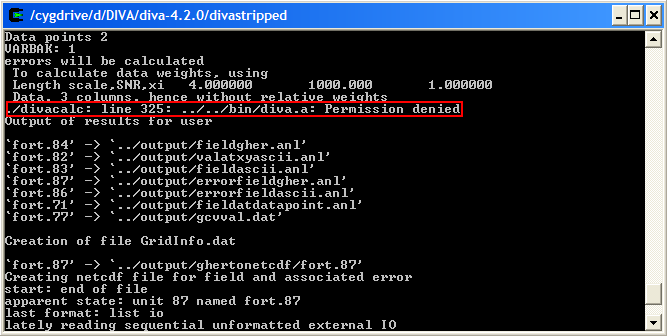
\includegraphics[width=.80\textwidth]{error_gfortran}
\caption{Error message during execution of \command{divacalc} with gfortran\label{fig:error_gfortran}.}
\end{figure}

\subsubsection{\question}
%--------------------------------------

Although the compilation worked without any message error, \texttt{diva.a} cannot be executed. This problem seems to occur only with \textsl{gfortran} compiler under \textsf{Cygwin}. Actually the problem is not related to permission (command \command{chmod} will not solve the problem) but with compilation. As described in problem \ref{sec:error_resource}, values of parameters\, \texttt{nrea} and \texttt{nent} shall be decreased and the sources recompiled.

\subsubsection{\answer}
%--------------------------

Same as problem \ref{sec:error_resource}. 


%------------------------------------------------------------------------------------


\subsection{Problem with contour generation}
%------------------------------------------

See Fig.~\ref{error:cont}.

\begin{figure}[htpb]
\centering
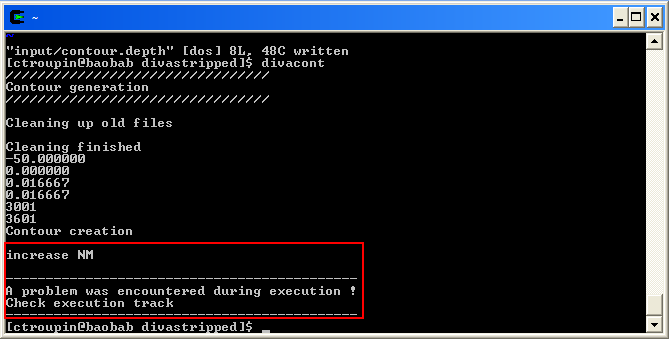
\includegraphics[width=.80\textwidth]{error_divacont}
\caption{Error message with contour generation.\label{error:cont}}
\end{figure}

\subsubsection{\question}
%---------------------

The number of contours created from a given topography (Section~\ref{sec:contourtopo}) is too high. 

\subsubsection{\answer}
%-------------------

Modify the first line of \file{contourgen.f} (located in \directory{./src/Fortran/Mesh/}) and increase the value of \texttt{nm}:
\begin{verbatim}
parameter(nm=5000000)
\end{verbatim}

\subsubsection{Additional information}
%----------------------------------

As the default value of \texttt{nm} is already large, you may also consider working with a topography with lower resolution. This should avoid the creation of of a great number of very small contours (e.g. Fig.~\ref{fig:smallcont}), which will not necessarily add quality to your analysis.


\begin{figure}[htpb]
\centering
\parbox{.65\textwidth}{
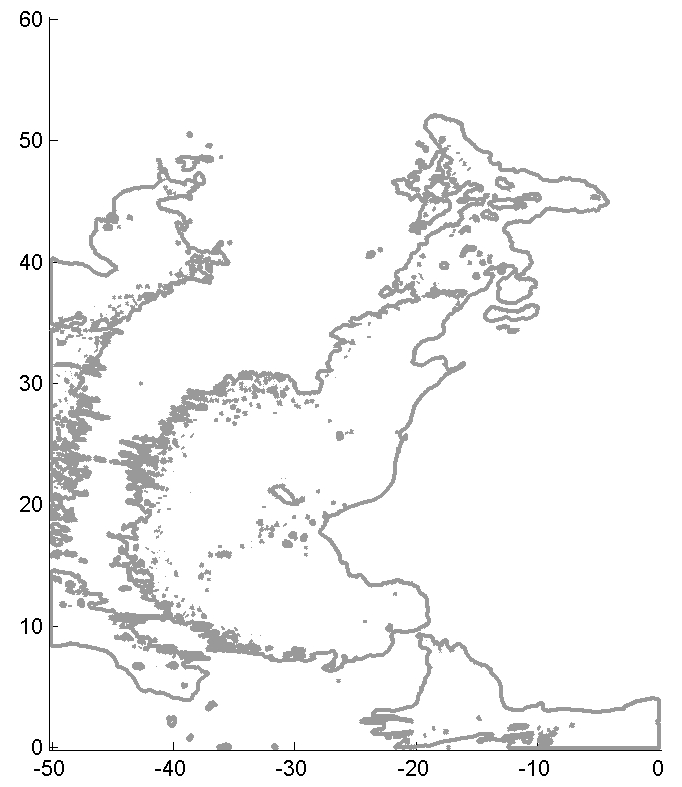
\includegraphics[width=.6\textwidth]{fine_contour}
}\parbox{.35\textwidth}{
\caption[Small contours]{Small contours created from DBDBV topography in the North Atlantic at 4500~m depth\label{fig:smallcont}.}
}
\end{figure}
 


%




%-------------------------------------------------------------------------------

\subsection{Analysis yields empty field}
%------------------------------------------


After the execution of \command{divacalc}, you get very small input files, with only one grid point.

\subsubsection{\question}
%--------------------------------------

The most frequent reason is that the \file{param.par} file has been modified during the execution of (Generalised) Cross Validation\index{Generalised Cross Validation} and the process was interrupted before it ends, leaving a parameter file similar to \ref{fig:errorparampar}. Note that in order to save computational time, \texttt{nx} and \texttt{ny} are set to $1$, since the analysis at every grid points is not necessary.

\begin{figure}[htpb]
\centering
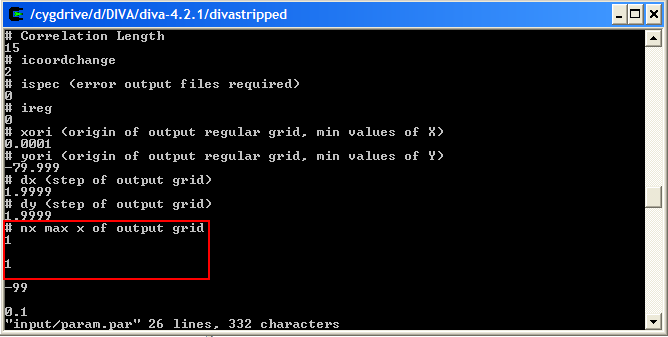
\includegraphics[width=.80\textwidth]{error_parampar}
\caption{File \file{param.par} resulting from an interruption of \command{divagcv}.\label{fig:errorparampar}}
\end{figure}

\subsubsection{\answer}
%--------------------------------------


Simply edit \file{param.par} to write the correct values of \texttt{nx} and \texttt{ny}, then run again \command{divacalc} (or \command{divadress}) to have an analysis on the desired grid.


\subsection{Windows runs out of virtual memory during diva execution}
%------------------------------------------


\subsubsection{\question}
%--------------------------------------

The problem arises probably because you have a computer with little RAM.

\diva uses a memory allocation for the largest problem encountered. This 
translates in Windows to a request of virtual memory of around 1.3~Gb.
During execution, the real memory used can be much smaller than that and 
the problem actually fit in real memory, even if you have less than 1~Gb RAM.

The only problem is that if your Windows virtual memory (the swap file) 
is not big enough, \diva will not execute.


\subsubsection{\answer}
%--------------------------------------

The best solution would be to 
add real memory (your computer would benefit from it anyway), but to 
make \diva work you can simply increase the virtual memory of Windows by 
changing the windows settings. As administrator:\\

\begin{verbatim}
my computer   right click
 -> properties  -> advanced -> performance
 -> settings -> advanced -> change
\end{verbatim}

Put there a virtual memory (swap file) of 2~Gb (initial and maximum) and 
\diva should run. 

Other solution consists of recompiling with lower \texttt{nrea} value (see problem~\ref{sec:error_compile}).


\subsection{"Cannot move directory" \ldots "permission denied" messages}
%------------------------------------


%\begin{figure}[htpb]
%\centering
%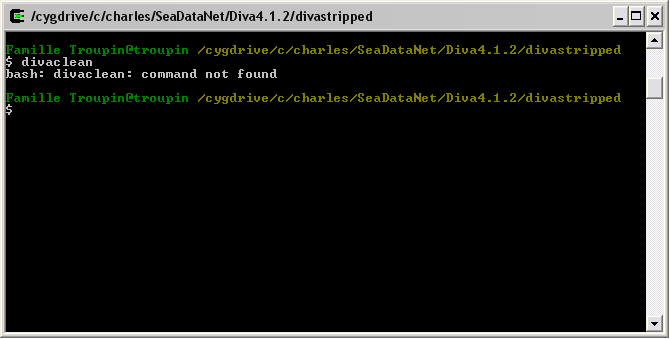
\includegraphics[width=.80\textwidth]{problempath}
%\caption{Error message when a command is not found.}
%\end{figure}

\subsubsection{\question}
%--------------------------------------

An application has opened one or several files located in the directory you want to (re)move, so that it is impossible to perform the operation.

\subsubsection{\answer}
%--------------------------------------

Simply close the application(s) that open the files of the concerned directory.


\section{Solved problems}
%------------------------


The following problems should not appear any more in the latest version of \diva. Should you encounter them, please contact us.

%--------------------------------------------------------------------------------------------------------------------------------------------

\subsection{Jacobian matrix with null determinant}
%------------------------------------------

The value of the Jacobian determinant is zero (Fig.~\ref{fig:error_jacobian}).
\begin{figure}[htpb]
\centering
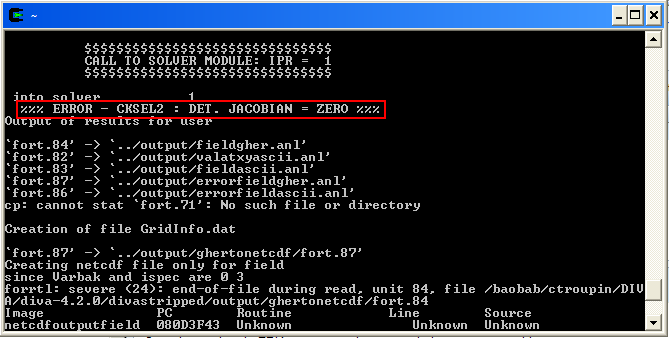
\includegraphics[width=.80\textwidth]{error_jacobian}\\
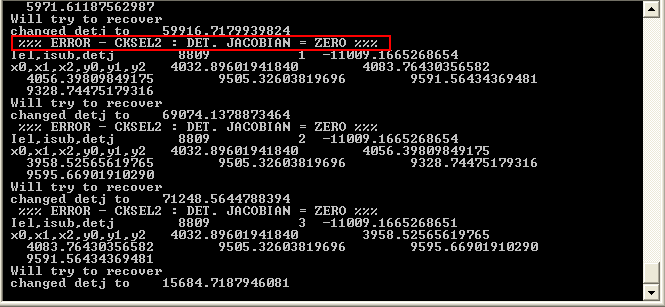
\includegraphics[width=.80\textwidth]{error_jacobian2}
\caption{Examples of \diva execution with problem with the Jacobian matrix. \label{fig:error_jacobian}}
\end{figure}

\subsubsection{\question}
%--------------------------------------

This messages comes from a problem in the mesh generation: some of the triangular elements are too deformed and generate a null value for the determinant. Then the solver cannot work, since it needs to inverse the Jacobian matrix.


\subsubsection{\answer}
%--------------------------------------

This problem was fixed in latest versions of \diva. 

-------------------------------------------------------------------------------

\subsection{Analysed field with white stripes}
%------------------------------------------

The analysed fields has stripes of $NaN$ values.

\begin{figure}[htpb]
\centering
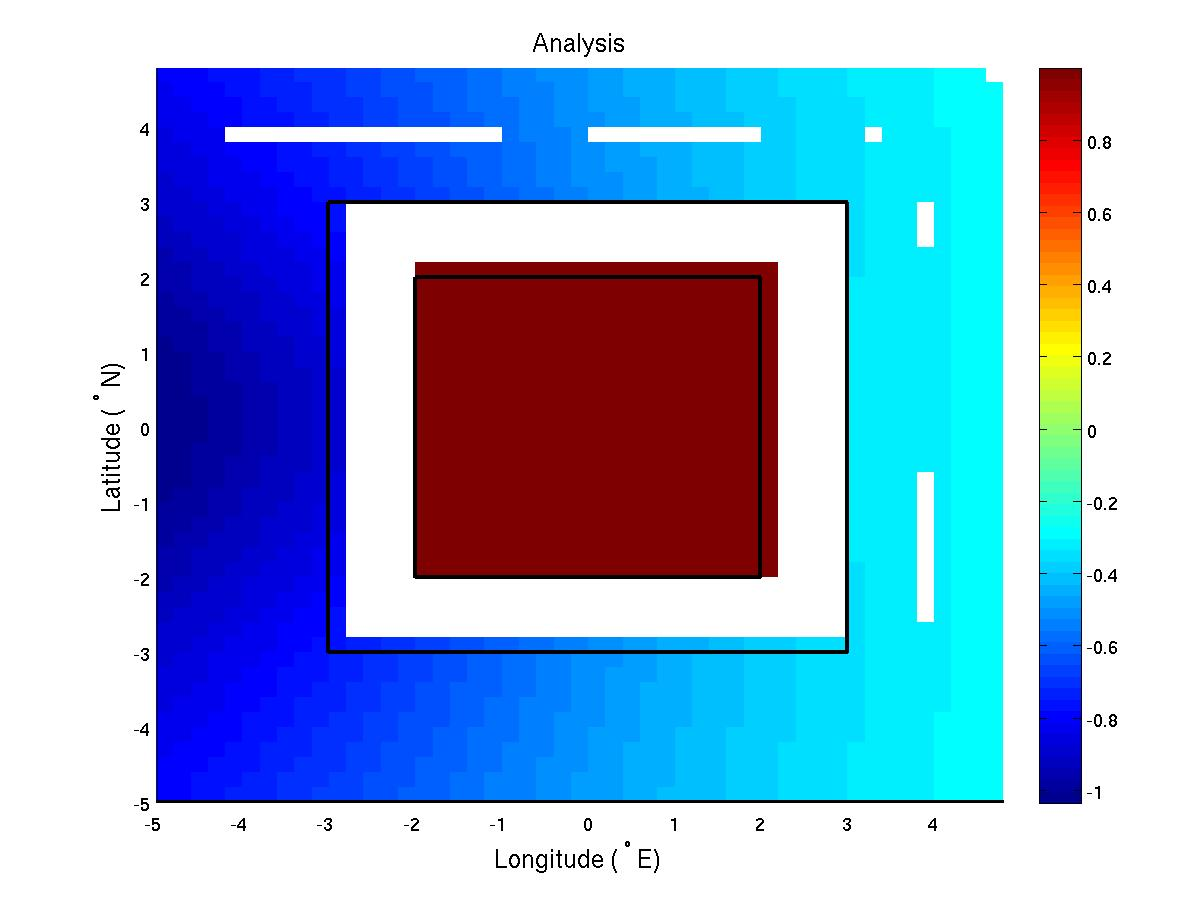
\includegraphics[width=.45\textwidth]{error_stripes}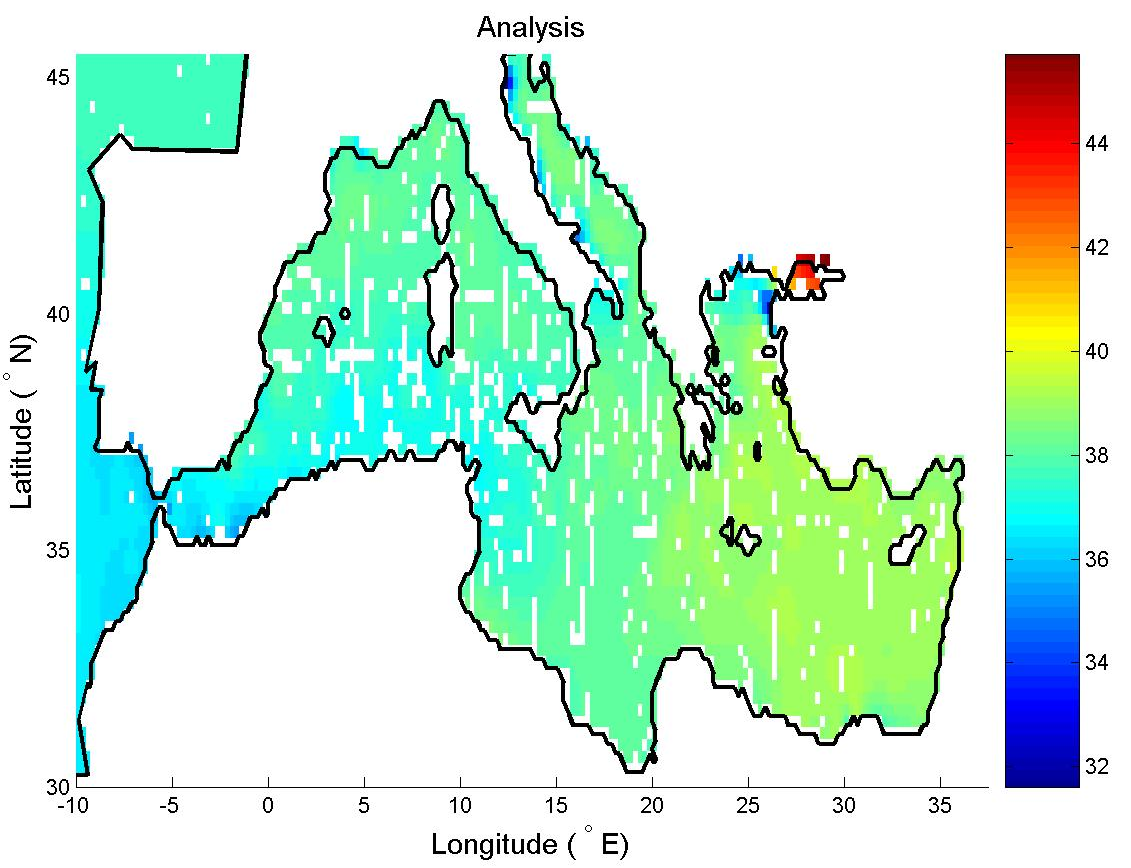
\includegraphics[width=.45\textwidth]{error_stripes3}
\caption{Examples of \diva outputs with random zones of $NaN$.\label{fig:error_stripes2}}
\end{figure}

\subsubsection{\question}
%--------------------------------------

This problem comes from a too aggressive optimisation to create executable \texttt{diva.a}, although during the compilation, no warning or error was issued.  

\subsubsection{\answer}
%--------------------------------------

This problem has been fixed in latest version of \diva. However, if you are still using older versions and get this kind of outputs, you can avoid them by changing the compilation flags and compile the source again. The recommended change is to use \texttt{'-O0'} flags instead of \texttt{'-O3'} (optimization flags) when compiling the sources located in the \directory{Fortran/Calc/} directory.


\subsection{"Corrupted data file" message}
%------------------------------------


\begin{figure}[htpb]
\centering
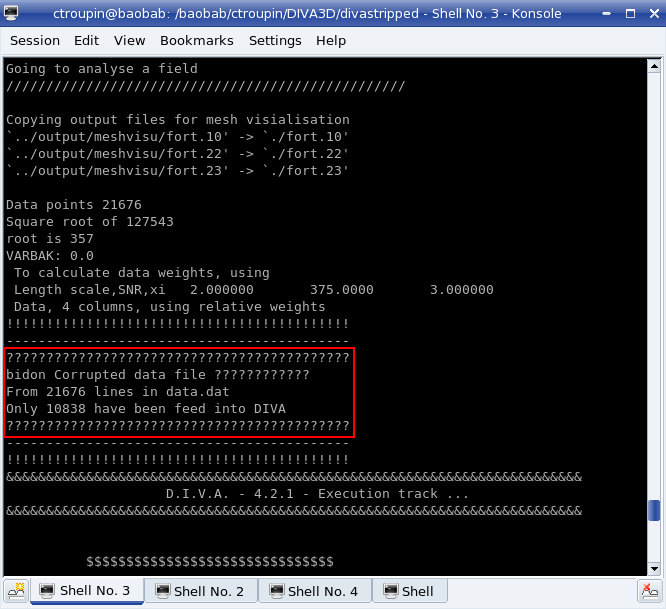
\includegraphics[width=.80\textwidth]{corrupted_file}
\caption{Error message during the reading of the data file.}
\end{figure}

\subsubsection{\question}
%--------------------------------------


This problem was observed when decimal numbers were written with commas instead of points.


\subsubsection{\answer}
%--------------------------------------

Simply convert the decimal separator (e.g. using the commands described in the beginning of Chapter~\ref{chap:general}).


\subsubsection{Additional information}
%-----------------------------------

The behaviour of \texttt{awk} is susceptible to change the points into commas when used in \command{awkfilter} or other routines. To fix the problem, simply replace

\texttt{gawk}

by

\texttt{LC\_ALL=C gawk}.

Remark: in latest versions of the code, this bug was fixed by adding 

\texttt{export LC\_ALL=C}

in the scripts employing \texttt{awk}.